\section{External Interface Requirements}
\label{sec:External Interface Requirements}%

\subsection{User Interfaces}
\label{sec:user interfaces}%
In this subsection we provide some mockups that show an example of some possible user interface, one for the mobile app which will be available to the users and one for the web app available to the businesses, that offer the charging service.

\paragraph{EVD interaction with the mobile app of the eMall}
The EVD needs to download the mobile app on his cellphone in order to interact with the eMall and take advantage of its functionalities. The Graphical User Interface (GUI) of the application is thought as an user-friendly interface, to facilitate everyone in using the service. In this first mockup we see the initial page of the system, shown to the user when opening the application.
\begin{figure}[H]
    \centering
    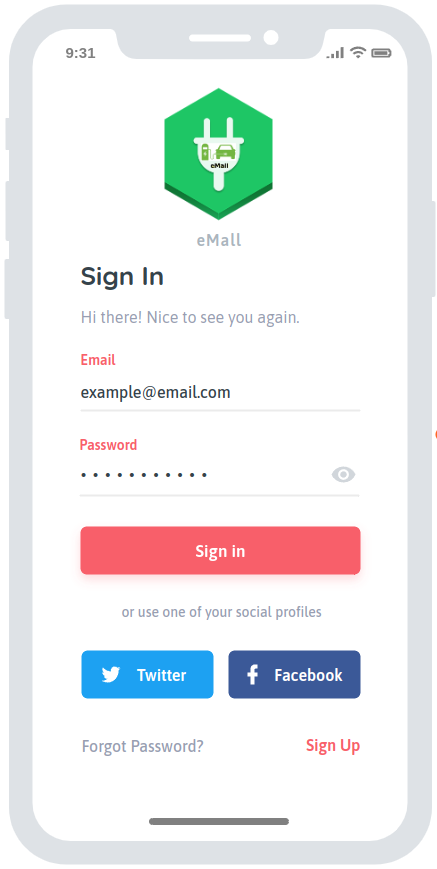
\includegraphics[scale=.3]{Images/cp3/signIn.png}
    \caption{Wireframe of the page that allows to log in from the eMma}
\end{figure}

In the following mockups we represent an example of the signing up procedure, showing the data required by the eMma in order to complete the creation of an account. 
\begin{figure}[H]
    \centering
    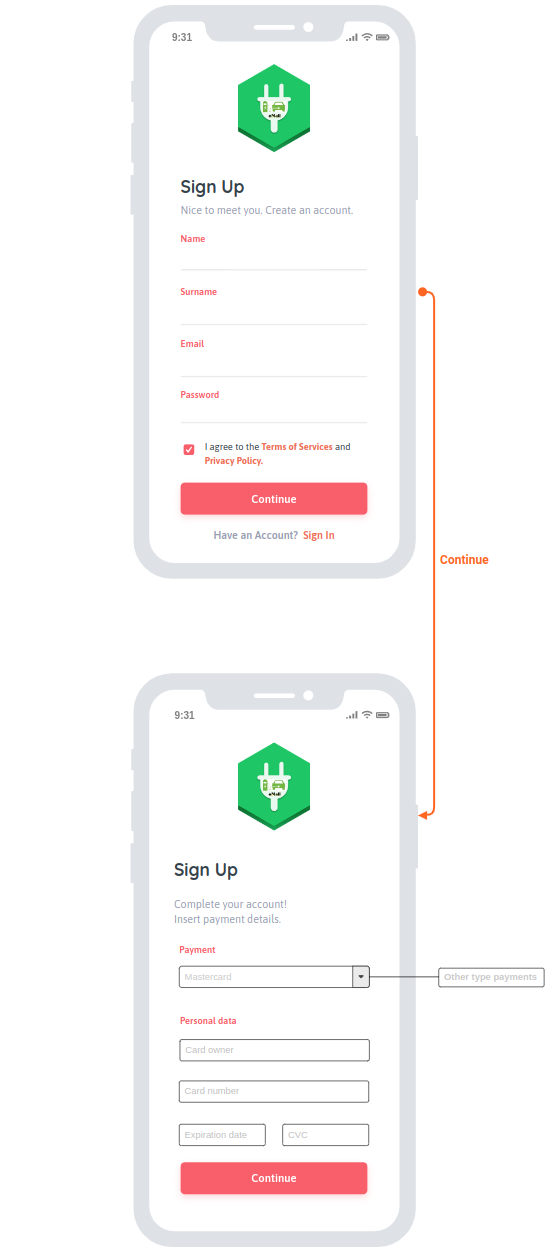
\includegraphics[scale=.45]{Images/cp3/signUp.png}
    \caption{Wireframe of the signing up process that allows to register from the eMma}
\end{figure}

\paragraph{CPO interaction with the managerial web app of the eMall}



\subsection{Hardware Interfaces}
\subsection{Software Interfaces}
\subsection{Communication Interfaces}

\section{Functional Requirements}
\label{sec:Functional Requirements}%

\section{Performance Requirements}
\label{sec:Performance Requirements}%

\section{Design Constraints}
\label{sec:Design Constraints}%

\subsection{Standards compliance}
\subsection{Hardware limitations}
\subsection{Any other constraint}

\section{Software System Attributes}
\label{sec:Software System Attributes}%

\subsection{Reliability}
\subsection{Availability}
\subsection{Security}
\subsection{Maintainability}
\subsection{Portability}

\clearpage
\section{EVD requirements traceability}
For the EVD requirements traceability we use the following acronyms for the components of the mapping:
\begin{itemize}
    \item eMma
    \item eMci
    \item ERH - EVDRequestHandler
    \item ERS - EVDRegistrationService
    \item CHS - ChargingHistoryService
    \item PS - PaymentService
    \item CSS - ChargingSessionService
    \item CSDM - ChargingStationDataManager
    \item BS - BookingService
    \item EPM - EVDProfileManager
    \item NS - NotificationService
    \item AS - AuthenticationService
    \item AL/DB - Database Abstraction Layer/Database Management System
\end{itemize}
Component from the CPMS\footnote{If an external CPMS is used, then wherever these component are cited in the matrix the external CPMS can be used instead}
\begin{itemize}
    \item CMS - CentralManagementService
    \item RS - ReservationService
    \item CSIS - ChargingStationInformationService
\end{itemize}
\begin{landscape}
\begin{center}
    \begin{longtable}[H]{
        |p{0.03\linewidth}
        |p{0.05\linewidth}
        |p{0.045\linewidth}
        |p{0.045\linewidth}
        |p{0.04\linewidth}
        |p{0.035\linewidth}
        |p{0.025\linewidth}
        |p{0.035\linewidth}
        |p{0.055\linewidth}
        |p{0.025\linewidth}
        |p{0.04\linewidth}
        |p{0.025\linewidth}
        |p{0.025\linewidth}
        |p{0.06\linewidth}
        |p{0.045\linewidth}
        |p{0.025\linewidth}
        |p{0.04\linewidth}|
        }
     \hline
     \textbf{R} & 
     %Components
     \textbf{eMma} &
     \textbf{eMci} &
     \textbf{ERH} &
     \textbf{ERS} & 
     \textbf{CHS} & 
     \textbf{PS} & 
     \textbf{CSS} & 
     \textbf{CSDM} &
     \textbf{BS} &
     \textbf{EPM} &
     \textbf{NS} &
     \textbf{AS} &
     \textbf{AL/DB} &
     \textbf{CMS} &
     \textbf{RS} &
     \textbf{CSIS} \\
     \hline

R1& x& & x& x& & & & & & & & x& & & & \\
\hline
R2& x& & x& & & & & & & x& & & & & & \\
\hline
R3& x& & x& & & & & & & x& & & x& & & \\
\hline
R4& x& & x& & & & & & & x& & & x& & & \\
\hline
R5& x& & x& & & & & & & x& & & x& & & \\
\hline
R6& x& & x& & & & & & & x& & & x& & & \\
\hline
R7& x& & x& & & & & & & x& & & x& & & \\
\hline
R8& x& & x& & & & & x& & & & & x& & & x\\
\hline
R9& x& & x& & & & & x& & & & & x& & & x\\
\hline
R10& x& & x& & & & & x& & & & & x& & & x\\
\hline
R11& x& & x& & & & & x& & & & & x& & & x\\
\hline
R12& x& & x& & & & & x& & & & & x& & & x\\
\hline
R13& x& & x& & & & & x& & & & & x& & & \\
\hline
R14& x& & & & & & & & & & & & & & & \\
\hline
R15& x& & & & & & & & & & & & & & & \\
\hline
R16& x& & & & & & & & & & & & & & & \\
\hline
R17& x& & x& & & & & x& x& & & & x& & x& \\
\hline
R18& x& & x& & & & & & x& & & & x& & x& \\
\hline
R19& x& & x& & & & & & x& & & & x& & x& \\
\hline
R20& x& & x& & & & & & & x& & & x& & & \\
\hline
R21& x& & x& & x& & & & & & & & x& & & \\
\hline
R22& x& & x& & x& & & & & & & & x& & & \\
\hline
R23& x& & x& & & & x& & & & & & x& x& & \\
\hline
     \textbf{R} & 
     %Components
     \textbf{eMma} &
     \textbf{eMci} &
     \textbf{ERH} &
     \textbf{ERS} & 
     \textbf{CHS} & 
     \textbf{PS} & 
     \textbf{CSS} & 
     \textbf{CSDM} &
     \textbf{BS} &
     \textbf{EPM} &
     \textbf{NS} &
     \textbf{AS} &
     \textbf{AL/DB} &
     \textbf{CMS} &
     \textbf{RS} &
     \textbf{CSIS} \\
     \hline
R24& x& x& & & & & & & & & & & & & & \\
\hline
R25& x& & x& & & x& & & & & & & & & & \\
\hline
R26& x& & x& & & & & & & & & x& & & & \\
\hline
R28& x& & & & & & & & & & & & & & & \\
\hline
R29& & & & & x& & x& & x& & & & x& & & \\
\hline
R31& & & & & & & & x& & & & & x& & & x\\
\hline
R32& x& & & x& x& x& x& x& x& x& x& & & & & \\
\hline
R33& x& & x& x& x& x& x& x& x& x& x& & & & & \\
\hline
R34& x& & & & & & & & & & & & & & & \\
\hline
R35& x& & & & & & & & & & & & & & & \\
\hline
R36& x& & & x& & x& x& x& x& x& & & x& & & \\
\hline
R37& x& & x& & & & & x& & & & & x& & & x\\
\hline
R38& x& & x& & & & & x& & & & & x& & & x\\
\hline
R39& x& & & & & & & & & & & & & & & \\
\hline
R40& & & & & & & x& x& & & & & x& & & x\\
\hline
R41& & & & & & & & & & & & & & x& & \\
\hline

     
    \caption{EVD's requirements traceability matrix}
    \label{tab:EVD requirements traceability }
    \end{longtable}
\end{center}
\end{landscape}


\subsubsection{EVD requirements traceability explanation}
Let us start the description of the traceability matrix for the EVD requirements by pointing out that the component EVDRequestHandler is required every time the user makes a request to the system, so it is present in most of  requirements. The same can be said for eMma, since it is responsible for interacting with the user. Hence, in the following paragraphs we will omit describing these component in each requirements they collaborate on satisfying. Moreover we have considered the eMSPRequestHandler since all the request to the CPMS components pass through it, this implies that every time a CPMS component maps to a requirement there is also the eMSPRequestHandler.\\
\\
\textbf{R1: The system shall allow an unregistered EVD to register an account}
\begin{itemize}
	\item eMma
	\item EVDRequestHandler
	\item EVDRegistrationService
	\item AuthenticationService
\end{itemize}
To allow an EVD to register we need eMma for handling the user interaction and view, the EVDRequestHandler, as said before, to receive the requests from eMma and forward them to the right components. The EVDRegistrationService is the main micro-service which handles most of the registration process and uses the AuthenticationService to validate the user credentials and handles them in a secure manner.\\
\\
The requirements concerned with the user management of his personal data (R2-R7) are all solved by the EVDProfileManager. After the user interacts with eMma and selects the modification he wants to do, the request is forwarded to the eMSP. Here is analyzed by the EVDRequestHandler which assigns it to the EVDProfileManager. Obviously the data must be stored and retrieved from a DB, hence the presence of the DBAL and DBMS.\\
\\
\textbf{R2: The system shall allow a registered EVD to insert data about his EVs}
\begin{itemize}
	\item eMma
	\item EVDRequestHandler
	\item EVDProfileManager
    \item Database Abstraction Layer/Database Management System
\end{itemize}
 
\textbf{R3: The system shall allow a registered EVD to update EV’s details}
\begin{itemize}
	\item eMma
	\item EVDRequestHandler
	\item EVDProfileManager
    \item Database Abstraction Layer/Database Management System
\end{itemize}

\textbf{R4: The system shall allow a registered EVD to add new EVs}
\begin{itemize}
	\item eMma
	\item EVDRequestHandler
	\item EVDProfileManager
    \item Database Abstraction Layer/Database Management System
\end{itemize}

\textbf{R5: The system shall allow a registered EVD to delete an EV}
\begin{itemize}
	\item eMma
	\item EVDRequestHandler
	\item EVDProfileManager
    \item Database Abstraction Layer/Database Management System
\end{itemize}

\textbf{R6: The system shall allow a registered EVD to insert personal data (name, surname, email, payment details)}
\begin{itemize}
	\item eMma
	\item EVDRequestHandler
	\item EVDProfileManager
    \item Database Abstraction Layer/Database Management System
\end{itemize}

\textbf{R7: The system shall allow a registered EVD to update personal data}
\begin{itemize}
	\item eMma
	\item EVDRequestHandler
	\item EVDProfileManager
    \item Database Abstraction Layer/Database Management System
\end{itemize}

To provide EVDs with information about the charging stations (such as price, promotions, type of charging point) (R8-R13) we envisioned the component ChargingStationDataManager to handle this operation. The component will periodically query information about charging stations from their respective CPMS and store them in the DBMS. When the user wants to know information about charging stations, the ChargingStationManager shall retrieve the appropriate information from the DB and send them back to the user as a reply. From the perspective of the CPMS, the component responsible for granting this information is he ChargingStationInformationService\\
\\
\textbf{R8: The system shall allow an EVD to view the charging stations on the map}
\begin{itemize}
	\item eMma
	\item EVDRequestHandler
	\item ChargingStationDataManager
    \item ChargingStationInformationService
	\item Database Abstraction Layer/Database Management System
\end{itemize}

\textbf{R9: The system shall allow an EVD to view relevant data about the charging stations}
\begin{itemize}
	\item eMma
	\item EVDRequestHandler
	\item ChargingStationDataManager
    \item ChargingStationInformationService
	\item Database Abstraction Layer/Database Management System
\end{itemize}

\textbf{R10: The system shall allow an EVD to view relevant data about a specific charging point}
\begin{itemize}
	\item eMma
	\item EVDRequestHandler
	\item ChargingStationDataManager
    \item ChargingStationInformationService
	\item Database Abstraction Layer/Database Management System
\end{itemize}

\textbf{R11: The system shall allow an EVD to view the prices of the charging points of the stations}
\begin{itemize}
	\item eMma
	\item EVDRequestHandler
	\item ChargingStationDataManager
    \item ChargingStationInformationService
	\item Database Abstraction Layer/Database Management System
\end{itemize}

\textbf{R12: The system shall allow an EVD to view the special offers of the charging points of the stations}
\begin{itemize}
	\item eMma
	\item EVDRequestHandler
	\item ChargingStationDataManager
    \item ChargingStationInformationService
	\item Database Abstraction Layer/Database Management System
\end{itemize}

\textbf{R13: The system shall allow a registered EVD to review a charging station}
\begin{itemize}
	\item eMma
	\item EVDRequestHandler
	\item ChargingStationDataManager
	\item Database Abstraction Layer/Database Management System
\end{itemize}

\textbf{R14: The system shall allow an EVD to share his location through the GPS module of his mobile phone}
\begin{itemize}
	\item eMma
\end{itemize}
To allow the user to share his location through GPS module, the eMma component, which is an application running on the user smartphone, will interact with the GPS module on the user smartphone to get the location data.\\
\\
\textbf{R15: The system shall allow an EVD to choose the area in which to visualize the charging stations on the map, if different from the actual GPS
location}
\begin{itemize}
	\item eMma
\end{itemize}
This feature will be offered by eMma, the user can select a different area from his actual location and eMma will make the request to the eMSP server accordingly.\\
\textbf{R16: The system by default must show on the homepage the charging stations on the map territory, centered on the EVD’s location}
\begin{itemize}
	\item eMma
\end{itemize}
As we already explained in the mapping of the previous requirement, eMma will interact with the GPS module of the EVD's smartphone to provide the user with location based services. If the user doesn't change any settings, eMma will, by default, show the charging station nearby to the EVD's location.\\
\\
\textbf{R17: The system shall allow a registered EVD to book a charge from an available charging point in a charging station}
\begin{itemize}
	\item eMma
	\item EVDRequestHandler
	\item ChargingStationDataManager
	\item BookingService
	\item Database Abstraction Layer/Database Management System
	\item ReservationService
\end{itemize}
To book a charging session in a charging point from a specific station, the EVD has to insert the appropriate information in the eMma terminal. The request will then be handled by the BookingService component of the eMSP, which after a preliminary consistency check of the information the user has inserted with the ones the system has saved locally, it will retrieve the information necessary to communicate with the appropriate CPMS and forward it the reservation request. On the CPMS side, the request will be handled by the ReservationService, which after his consistency check will confirm the reservation or deny it.\\
\\
\textbf{R18: The system shall allow a registered EVD to choose the time-frame (date and time) in which to book a charge}
\begin{itemize}
	\item eMma
	\item EVDRequestHandler
	\item BookingService
	\item Database Abstraction Layer/Database Management System
	\item ReservationService
\end{itemize}
This functionality is granted by the component we previously discussed in the mapping of requirement R18. The user has to just insert the time-frame from the eMma terminal, then the request will be handled by these components.\\
\\
\textbf{R19: The system shall allow a registered EVD to cancel a charging point booking}
\begin{itemize}
	\item eMma
	\item EVDRequestHandler
	\item BookingService
	\item Database Abstraction Layer/Database Management System
	\item ReservationService
\end{itemize}
The components which collaborate to offer this functionality are still the ones mentioned in the two previous mappings. The flow of interaction is totally similar to the one seen for R17.\\
\\
\textbf{R20: The system shall allow a registered EVD to visualize his profile data}
\begin{itemize}
	\item eMma
	\item EVDRequestHandler
	\item EVDProfileManager
    \item Database Abstraction Layer/Database Management System
\end{itemize}
The component responsible to show the user his profile data is mainly the eMma. If eMma hasn't stored locally the user profile data, it must request them to the eMSP. The request will be handled by the EVDProfileManager which will retrieve the information from the DB.\\
\\
\textbf{R21: The system shall allow a registered EVD to view the charging history}
\begin{itemize}
	\item eMma
	\item EVDRequestHandler
	\item ChargingHistoryService
	\item Database Abstraction Layer/Database Management System
\end{itemize}
This interaction is totally similar to the previous one, except for the fact that for this specific case the component responsible for retrieving and delivering the data in the eMSP is the ChargingHistoryService.\\
\\
\textbf{R22: The system shall allow a registered EVD to choose a visualization criteria for the charging history}
\begin{itemize}
	\item eMma
	\item EVDRequestHandler
	\item ChargingHistoryService
    \item Database Abstraction Layer/Database Management System
\end{itemize}
As this operation involves the manipulation of information about the charging history the component responsible for handling this request is obviously the ChargingHistoryService.\\
\\
To start a charging session the user needs to fetch the code shown by the eMci terminal on the charging point (R24) and insert it in the eMma mobile application, this code uniquely identifies the charging point. The request is then passed to the ChargingSessionService, which will check the correctness of the code before forwarding the request to the corresponding CPMS. Here, the request is handled by the CentralManagementService, which will unlock the charging point and enable the flow of electricity if the data from the eMSP are correct.\\

\textbf{R23: The system shall allow an EVD to start a charging session}
\begin{itemize}
	\item eMma
	\item EVDRequestHandler
	\item ChargingSessionService
    \item Database Abstraction Layer/Database Management System
	\item CentralManagementService
\end{itemize}

\textbf{R24: The system shall allow a registered EVD to insert the charging point code, in order to start a charging session}
\begin{itemize}
	\item eMma
	\item eMci
\end{itemize}

\textbf{R25: The system shall allow an EVD to choose the payment method to use in order to pay for the obtained service}
\begin{itemize}
	\item eMma
	\item EVDRequestHandler
	\item PaymentService
\end{itemize}
The user can select a payment method, from one of those supported by the system, directly from the eMma. The eMma will require the EVD to enter all the necessary details to process the payment request. All the data will then passed to PaymentService micro-services which will interact with the specific payment processor indicate by the EVD, through the exposed API to complete the payment process.\\\\
\textbf{R26: The system must allow the registered EVD to log in}
\begin{itemize}
	\item eMma
	\item EVDRequestHandler
	\item AuthenticationService
\end{itemize}
To login into the system the EVD must insert his credentials in eMma. This credentials will then be validated by the AuthenticationService, which will return a token to be used for the request that need authorization.\\\\
\textbf{R28: The system must allow the EVD to access the mobile application, eMma, with or without an account}
\begin{itemize}
	\item eMma
\end{itemize}
The eMma shall be built in a such way that some of the functionalities can be accessed even without logging in the system.\\\\
\textbf{R29: The system must store the charging history: previous charges and bookings related to the specific EV}
\begin{itemize}
	\item ChargingHistoryService
        \item ChargingSessionService
        \item BookingService
	\item Database Abstraction Layer/Database Management System
\end{itemize}
To have a charging history of bookings and charging sessions each of the components responsible for handling the charging sessions and bookings, ChargingSessionService and BookingService respectively, shall save the data of the session or booking on the DB. Then the Charging history component will be responsible for processing this data in the right format.\\
\\
\textbf{R31: The system must collect the data about the charging stations from the CPOs}
\begin{itemize}
	\item ChargingStationDataManager
	\item Database Abstraction Layer/Database Management System
\end{itemize}
The task of collecting the data from the charging stations managed by different CPOs is entrusted to the ChargingStationDataManager. This component periodically queries the CPMS, that knows about the information of the managed charging stations.\\
\\
Whenever an error occurs during the request of the service the micro-service handling that request must return an error message containing the specifics of the error. Afterwards eMma will be responsible of showing the error message to the user. On the other hand (R33), if the operations terminates successfully, then, eMma shall notify the user about the correct conclusion of the operation. If the component needs to send a notification to user, even if the user is waiting for a reply, it will be used the NotificationService component.\\
\\
\textbf{R32: The system must notify the EVD with a specific message, that clarifies the problem, if an error occurs (login error, update error, payment error, ecc.)}
\begin{itemize}
	\item eMma
	\item EVDRegistrationService
	\item ChargingHistoryService
	\item PaymentService
	\item ChargingSessionService
	\item ChargingStationDataManager
	\item BookingService
	\item EVDProfileManager
	\item NotificationService
\end{itemize}

\textbf{R33: The system must notify the EVD with a success message if the operation terminated without errors (successful registration, successful profile modification, ecc.)}
\begin{itemize}
	\item eMma
	\item EVDRequestHandler
	\item EVDRegistrationService
	\item ChargingHistoryService
	\item PaymentService
	\item ChargingSessionService
	\item ChargingStationDataManager
	\item BookingService
	\item EVDProfileManager
	\item NotificationService
\end{itemize}

The following requirements (R34-R35) are satisfied by eMma, which must not allow the user to perform any request before giving consent. \\
\textbf{R34: The system must ask for EVD’s consent to use the location information
given by the GPS module}
\begin{itemize}
	\item eMma
\end{itemize}

\textbf{R35: The system must ask the EVD, during registration, to agree to the terms
of service}
\begin{itemize}
	\item eMma
\end{itemize}

\textbf{R36: The system must check for the correctness of the data inserted by the
EVD (login details, charging point code, etc.)}
\begin{itemize}
	\item eMma
	\item EVDRegistrationService
	\item PaymentService
	\item ChargingSessionService
	\item ChargingStationDataManager
	\item BookingService
	\item EVDProfileManager
\end{itemize}
Each component shall check the correctness of the provided data before executing the request.\\
\\
\textbf{R37: The system must show only the free charging points to book}
\begin{itemize}
	\item eMma
	\item EVDRequestHandler
	\item ChargingStationDataManager
	\item Database Abstraction Layer/Database Management System
\end{itemize}
The information about free charging points is managed by the ChargingStationDataManager, which will return to eMma this information in an appropriate data structure. eMma is responsible to show to the user this information.\\
\\
\textbf{R38: The system must show for each available charging point the relevant
information (type of charging, type of socket, charging speed, price,
special offers, etc.)}
\begin{itemize}
	\item eMma
	\item EVDRequestHandler
	\item ChargingStationDataManager
	\item Database Abstraction Layer/Database Management System
\end{itemize}
As we said before, the component responsible for managing the data about the charging stations and charging points is the ChargingStationDataManager. This component shall save the data about the charging point in the DB, from which it can retrieve in the future and send back to eMma when it requests them.\\
\\
\textbf{R39: The system must show a summary of the successful booking operation}
\begin{itemize}
	\item eMma
\end{itemize}
When eMma receives the booking confirmation from the BookingService, it must show a summary of the booking.\\
\\
\textbf{R40: The system must change the status of the charging point during charging}
\begin{itemize}
	\item ChargingSessionService
	\item ChargingStationDataManager
    \item ChargingStationInformationService
	\item Database Abstraction Layer/Database Management System
\end{itemize}
When the user successfully unlocks the charging point, the ChargingSessionService must communicate this event to the ChargingStationDataManager, which will update it's internal information by setting the corresponding charging point as occupied. The CPMS must also execute this operation so to display to other eMSPs that the charging point is occupied. The component responsible for this in the CPMS is the ChargingStationInformationService.\\
\\
\textbf{R41: The system must unlock the charging point if the code is correct}
\begin{itemize}
	\item CentralManagementService
\end{itemize}
When the CentralManagementService (component of the CPMS) receives a request for unlocking a charging point with a correct code it must abide by the request enabling the flow of electricity for the chosen charging point.

\clearpage
\section{CPO requirements traceability}
For the CPO requirements traceability we use the following acronyms for the components of the mapping:
\begin{itemize}
    \item ANS - AnalyticsService
    \item SV - StationsVisualizer
    \item CSM - ChargingStationManager
    \item BMS - BatteryManagementService
    \item DMS - DSOManagementService
    \item NS - NotificationService
    \item AS - AuthenticationService
    \item AL/DB - Database Abstraction Layer/Database Management System
\end{itemize}
\begin{center}
    \begin{longtable}[H]{|p{0.05\linewidth}|p{0.075\linewidth}|p{0.075\linewidth}|p{0.075\linewidth}|p{0.075\linewidth}|p{0.075\linewidth}|p{0.075\linewidth}|p{0.075\linewidth}|p{0.085\linewidth}|}
     \hline
     \textbf{R} & 
     %Components
     \textbf{AS} & 
     \textbf{ANS} & 
     \textbf{SV} & 
     \textbf{CSM} & 
     \textbf{BMS} & 
     \textbf{DMS} & 
     \textbf{NS} & 
     \textbf{AL/DB}\\
     \hline
     R27 & X & & & & & & & X \\
     \hline
     R30 & & & & X & & X & & X \\
     \hline
     R42 & & & X & & & & & X \\
     \hline
     R43 & & & & & & & X & X \\
     \hline
     R44 & & & X & X & & & & X \\
     \hline
     R45 & & & X & X & & & & X\\
     \hline
     R46 & & & X & X & & X & & X\\
     \hline
     R47 & & & X & X & & & & X\\
     \hline
     R48 & & & X & X & & & & X\\
     \hline
     R49 & & & X & X & & & & X\\
     \hline
     R50 & & & X & X & & & & X\\
     \hline
     R51 & & & & X & & & & X\\
     \hline
     R52 & & & & X & & & & X\\
     \hline
     R53 & & & & X & & & X & \\
     \hline
     R54 & & & & X & & & X & \\
     \hline
     R55 & & & X & X & & & & X\\
     \hline
     R56 & & & X & X & & X & & X\\
     \hline
     R57 & & & X & X & & X & & X\\
     \hline
     R58 & & & X & X & & X & & X\\
     \hline
     R59 & & & X & X & & X & & X\\
     \hline
     R60 & & & X & X & & & & X\\
     \hline
     R61 & & X & & & & & & X\\
     \hline
     R62 & & X & & & & & & X\\
     \hline
     R64 & & & X & X & & & X & X\\
     \hline
     R65 & & & & X & X & & & X\\
     \hline
     R66 & & & & X & X & & & X\\
     \hline
    \caption{CPO requirements traceability matrix}
    \label{tab:CPO requirements traceability}
    \end{longtable}
\end{center}
In the previous table the CPORequestHandler component is missing from the representation, because all the CPO requirements need this component to be full-field. Every request passes through this component, which sends it to the specific service that implements the demanded functionality. This micro-service mainly communicates with the ChargingStationManager, that invokes in order to satisfy the client requests.

\subsubsection{CPO's requirement traceability explanation}
In the final part of this section we report all the requirements with the respective components in order for the reader to have a more clear view of their relation and we also add a minimal explanation to clarify this connection.As before, the CPORequestHandler will not be listed in the following parts, to avoid redundancy, because it always present. Also the web app is part of all the interactions, being the presentation layer with which the CPO interacts.\\

\textbf{R27: The system must allow the CPO to log in with the company credentials}
\begin{itemize}
    \item AuthenticationService
    \item DBAL and DBMS
\end{itemize}
To log in the CPO inserts the company credentials (email and password), already present on the CPOsDB, and the web app passes the authentication request to the CPORequestHandler, which communicates with the AuthenticationService and receives a token, if the credentials are valid. The token will be used to interact with the system in order to forward authorized requests.
\pagebreak


\textbf{R42: The system shall allow the CPO to view the charging stations}
\begin{itemize}
    \item StationsVisualizer
    \item DBAL and DBMS
\end{itemize}
After the log in, the web app sends a request to visualize the charging stations the CPO has to manage, and the request arrives to the StationsVisualizer component, which interacts with the DB, using the abstraction layer, to retrieve the minimal data about the stations that the web app needs to show on the homepage.

\textbf{R43: The system shall allow the CPO to view any notification regarding the charging stations}
\begin{itemize}
    \item NotificationService
    \item DBAL and DBMS
\end{itemize}
After the log in, there is also a request to the NotificationService, which acquires any notification the system has automatically produced, thus, the CPO can manage to solve possible warnings.

\textbf{R44: The system shall allow the CPO to update the details of a charging station}
\begin{itemize}
    \item StationsVisualizer
    \item ChargingStationManager
    \item DBAL and DBMS
\end{itemize}
After visualizing the stations, the CPO can select one of them and change some parameters, updating the details through the ChargingStationManager functionalities. In mainly all the interactions with the ChargingStationManager the CPO starts from visualizing the stations on the homepage; and to complete the requests the system has to access the DB and get some data or insert some data, through the use of the DBAL and the DBMS. We will not mention again all these details in the following explanations, since the interaction is always the same.

\textbf{R55: The system shall allow the CPO to select a charging station}
\begin{itemize}
    \item StationsVisualizer
    \item ChargingStationManager
    \item DBAL and DBMS
\end{itemize}
As already explained before, after the log in, the CPO can visualize the stations and select one of them getting the form of the station with the respective information, in virtue of the interaction with the ChargingStationManager and the persistent data.\\
\\

From R45 to R50, plus R60, we need almost the same components. To delete or add a charging station or a charging point we need to interact with the ChargingStationManager. Also in adding a charging station is necessary to communicate with the DSOManagementService in order to set the DSO from which to acquire energy, as explained before. The rest of the details that we need to add or update, such as the price and the special offers are handled by the ChargingStationManager itself, which interacts with the DB. \\
\textbf{R45: The system shall allow the CPO to delete a charging station }
\begin{itemize}
    \item StationsVisualizer
    \item ChargingStationManager
    \item DBAL and DBMS
\end{itemize}

\textbf{R46: The system shall allow the CPO to add a charging station}
\begin{itemize}
    \item StationsVisualizer
    \item ChargingStationManager
    \item DSOManagementService
    \item DBAL and DBMS
\end{itemize}

\textbf{R47: The system shall allow the CPO to delete a charging point from a charging station}
\begin{itemize}
    \item StationsVisualizer
    \item ChargingStationManager
    \item DBAL and DBMS
\end{itemize}

\textbf{R48: The system shall allow the CPO to add a charging point to a charging station}
\begin{itemize}
    \item StationsVisualizer
    \item ChargingStationManager
    \item DBAL and DBMS
\end{itemize}

\textbf{R49: The system shall allow the CPO to set the price of the charging point}
\begin{itemize}
    \item StationsVisualizer
    \item ChargingStationManager
    \item DBAL and DBMS
\end{itemize}

\textbf{R50: The system shall allow the CPO to set a special offer for the charging point}
\begin{itemize}
    \item StationsVisualizer
    \item ChargingStationManager
    \item DBAL and DBMS
\end{itemize}

\textbf{R60: The system shall allow the CPO to set a special offer for the charging station}
\begin{itemize}
    \item StationsVisualizer
    \item ChargingStationManager
    \item DBAL and DBMS
\end{itemize}
\vspace{1.5cm}

\textbf{R51: The system must check the correctness of the data inserted by the CPO}
\begin{itemize}
    \item ChargingStationManager
    \item DBAL and DBMS
\end{itemize}
Every time the CPO inserts new data the ChargingStationManager checks their correctness, before invoking other components.

\textbf{R52: The system must store the data of the charging stations}
\begin{itemize}
    \item ChargingStationManager
    \item DBAL and DBMS
\end{itemize}
The ChargingStationManager is the main component that allows to manage the stations and their data, so every time there is an update or any kind of action that changes the stations data, this component interacts with the DBAL to store the new data on the DB or to update the previous stored information.\\

To notify the user of a successful operation or of an error (R53 and R54) in some situations the ChargingStationManager has to interact with the NotificationService, especially if the notification is spontaneous, deriving from the system that monitors the stations and the energy flow. In other situations, such as sending only a confirmation message, the ChargingStationManager can complete the operation by itself. \\ 
\textbf{R53: The system must notify the CPO with a specific message if an error occurs during an operation}
\begin{itemize}
    \item ChargingStationManager
    \item NotificationService
\end{itemize}

\textbf{R54: The system must notify the CPO with a success message if the operation terminates without errors}
\begin{itemize}
    \item ChargingStationManager
    \item NotificationService
\end{itemize}

\textbf{R64: The system shall allow the CPO to select a notification to solve it }
\begin{itemize}
    \item StationsVisualizer
    \item ChargingStationManager
    \item NotificationService
    \item DBAL and DBMS
\end{itemize}
Once selected a notification, the NotificationService interacts with the ChargingStationManager and opens the form of the station associated to the warning, thus the CPO can solve the problem.\\
\\
All the operations which involve data regarding the DSO (R56-R57-R58-R59) are passed from the ChargingStationManager to the DSOManagementService, that is a micro-service focused on the DSO parameters, so it can check more in detail if the CPO's updates are valid and also can show the renewed information of the DSOs. Thus, the CPO can visualize the new prices and special offers of the DSOs and can change from which one to acquire energy and from which energy source, in order to improve the business profit.
\textbf{R56: The system shall allow the CPO to view the DSO's updated prices for the energy sources}
\begin{itemize}
    \item StationsVisualizer
    \item ChargingStationManager
    \item DSOManagementService
    \item DBAL and DBMS
\end{itemize}

\textbf{R57: The system shall allow the CPO to view the DSO's special offers for the energy sources}
\begin{itemize}
    \item StationsVisualizer
    \item ChargingStationManager
    \item DSOManagementService
    \item DBAL and DBMS
\end{itemize}

\textbf{R58: The system shall allow the CPO to change the DSO of a charging station}
\begin{itemize}
    \item StationsVisualizer
    \item ChargingStationManager
    \item DSOManagementService
    \item DBAL and DBMS
\end{itemize}

\textbf{R59: The system shall allow the CPO to choose the DSO's energy source for the charging station}
\begin{itemize}
    \item StationsVisualizer
    \item ChargingStationManager
    \item DSOManagementService
    \item DBAL and DBMS
\end{itemize}

\textbf{R30: The system must collect electric energy data from the DSOs}
\begin{itemize}
    \item ChargingStationManager
    \item DSOManagementService
    \item DBAL and DBMS
\end{itemize}
To collect energy from the DSOs is necessary to send an outside request through the DSO API, and this is a task carried out by the DSOManagementService, which interacts with the ChargingStationManager to save on the DB the data of the used DSO. Thus, the ChargingStationManager has to interact with the persistent data of the stations and keep track of the DSO from which the specific central system is collecting electric energy.\\
The following two requirements allow to the CPO to analyse the stations, and the micro-service assigned to this task is the AnalyticsService. This component interacts with the database in order to create a graphical view of the stations, based on some criteria chosen by the CPO. It acquires the persistent data and processes it, thus, the CPO can track some behaviours and trends in the business operations.\\
\textbf{R61: The system shall allow the CPO to select some criteria to graphically visualize aspects of the charging stations}
\begin{itemize}
    \item AnalyticsService
    \item DBAL and DBMS
\end{itemize}

\textbf{R62: The system must show a graphical representation of some aspects of the charging stations}
\begin{itemize}
     \item AnalyticsService
    \item DBAL and DBMS
\end{itemize}
\vspace{1.5cm}

Finally, the CPMS server of the eMall also allows to the CPO to manage the battery of the station, if it is present. For this activity is necessary to interact with the BatteryManagementService, which checks if the battery is functional and keeps track of the battery level. Also there is a communication with the CentralManagementService of the charging station, that we didn't show in the CPO requirement traceability, but we mention here to clarify the interaction shown in the sequence diagram. The BatteryManagementService needs to send a message to the CentralManagementService to communicate with the battery of the station and physically start the charging of the battery or switch to battery use. We also report the ChargingStationManager, the DBAL and DBMS in the achievement of these requirements, since the ChargingStationManager is the one that invokes the BatteryManagementService and saves the changes on the DB.\\
\textbf{R65: The system shall allow the CPO to decide if for a charging station wants to store energy from the DSO in the battery of the station}
\begin{itemize}
    \item ChargingStationManager
    \item BatteryManagementService
    \item CentralManagementService
    \item DBAL and DBMS
\end{itemize}

\textbf{R66: The system shall allow the CPO to decide if for a charging station wants to use the battery or acquire energy from the DSO}
\begin{itemize}
    \item ChargingStationManager
    \item BatteryManagementService
    \item CentralManagementService
    \item DBAL and DBMS
\end{itemize}
